\documentclass[a4paper,12pt]{report}
\usepackage[portuguese]{babel}
\usepackage{graphicx}
\usepackage{amsmath}
\usepackage{geometry}
\usepackage{setspace}
\usepackage{titlesec}
\usepackage{tocloft}
\usepackage{longtable}
\usepackage{lipsum}
\usepackage{enumitem}
\usepackage{fontspec}  
\usepackage{xcolor}
\usepackage[hidelinks]{hyperref}
\usepackage{ragged2e}
\usepackage[natbibapa]{apacite} % Estilo APA para o natbib
\usepackage{url}

% Configuração da Margem e Espaçamento
\geometry{a4paper, margin=2.5cm}
\setstretch{1.5}

% Configuração de Fontes
\setmainfont{Times New Roman}

% Configuração de Títulos
\titleformat{\chapter}[block]{\normalfont\huge\bfseries}{\thechapter.}{20pt}{\centering}
\titleformat{\section}[block]{\normalfont\Large\bfseries}{\thesection}{1em}{}

% Configuração do Índice
\addto\captionsportuguese{%
	\renewcommand{\contentsname}{Índice}
}
\renewcommand{\cftchapfont}{\bfseries}
\renewcommand{\cftsecfont}{\normalfont}
\renewcommand{\cftsubsecfont}{\itshape}
\renewcommand{\cftchappagefont}{\bfseries}
\renewcommand{\cftsecleader}{\cftdotfill{\cftdotsep}}

% Configuração de Cores
\definecolor{barraazul}{RGB}{0, 51, 153}

% Referências
\addbibresource{referencias.bib} % Aponta para o arquivo de bibliografia

% Começar numeração romana
\pagenumbering{roman}

\begin{document}
	
	% Capa
	\begin{titlepage}
		\begin{flushleft}
			
\includegraphics[width=0.5\textwidth]{iscte.png}\\[1cm]
		\end{flushleft}
		\noindent
		\textcolor{barraazul}{\rule{\textwidth}{1mm}} % Barra azul
		\\[0.5cm]
		{\Huge \textbf{\centering Desenvolvimento de modelos preditivos com base em RNN}}\\[1.5cm]
		\noindent
		\textbf{Luís Ricardo Silva Inácio}\\
		\textbf{Número de Aluno: 129074}\\[2cm]
		\textbf{Mestrado em Inteligência Artificial}\\[1.5cm]
		\textbf{Orientador: Tozé Brito, Phd}\\
		\textbf{Coorientador: (se aplicável)}\\[3cm]
		\textbf{Outubro, 2024}
	\end{titlepage}
	
	% Página em Branco
	\newpage
	\thispagestyle{empty}
	\mbox{}
	\newpage
	
	% Contracapa
	\begin{titlepage}
		\begin{flushleft}
			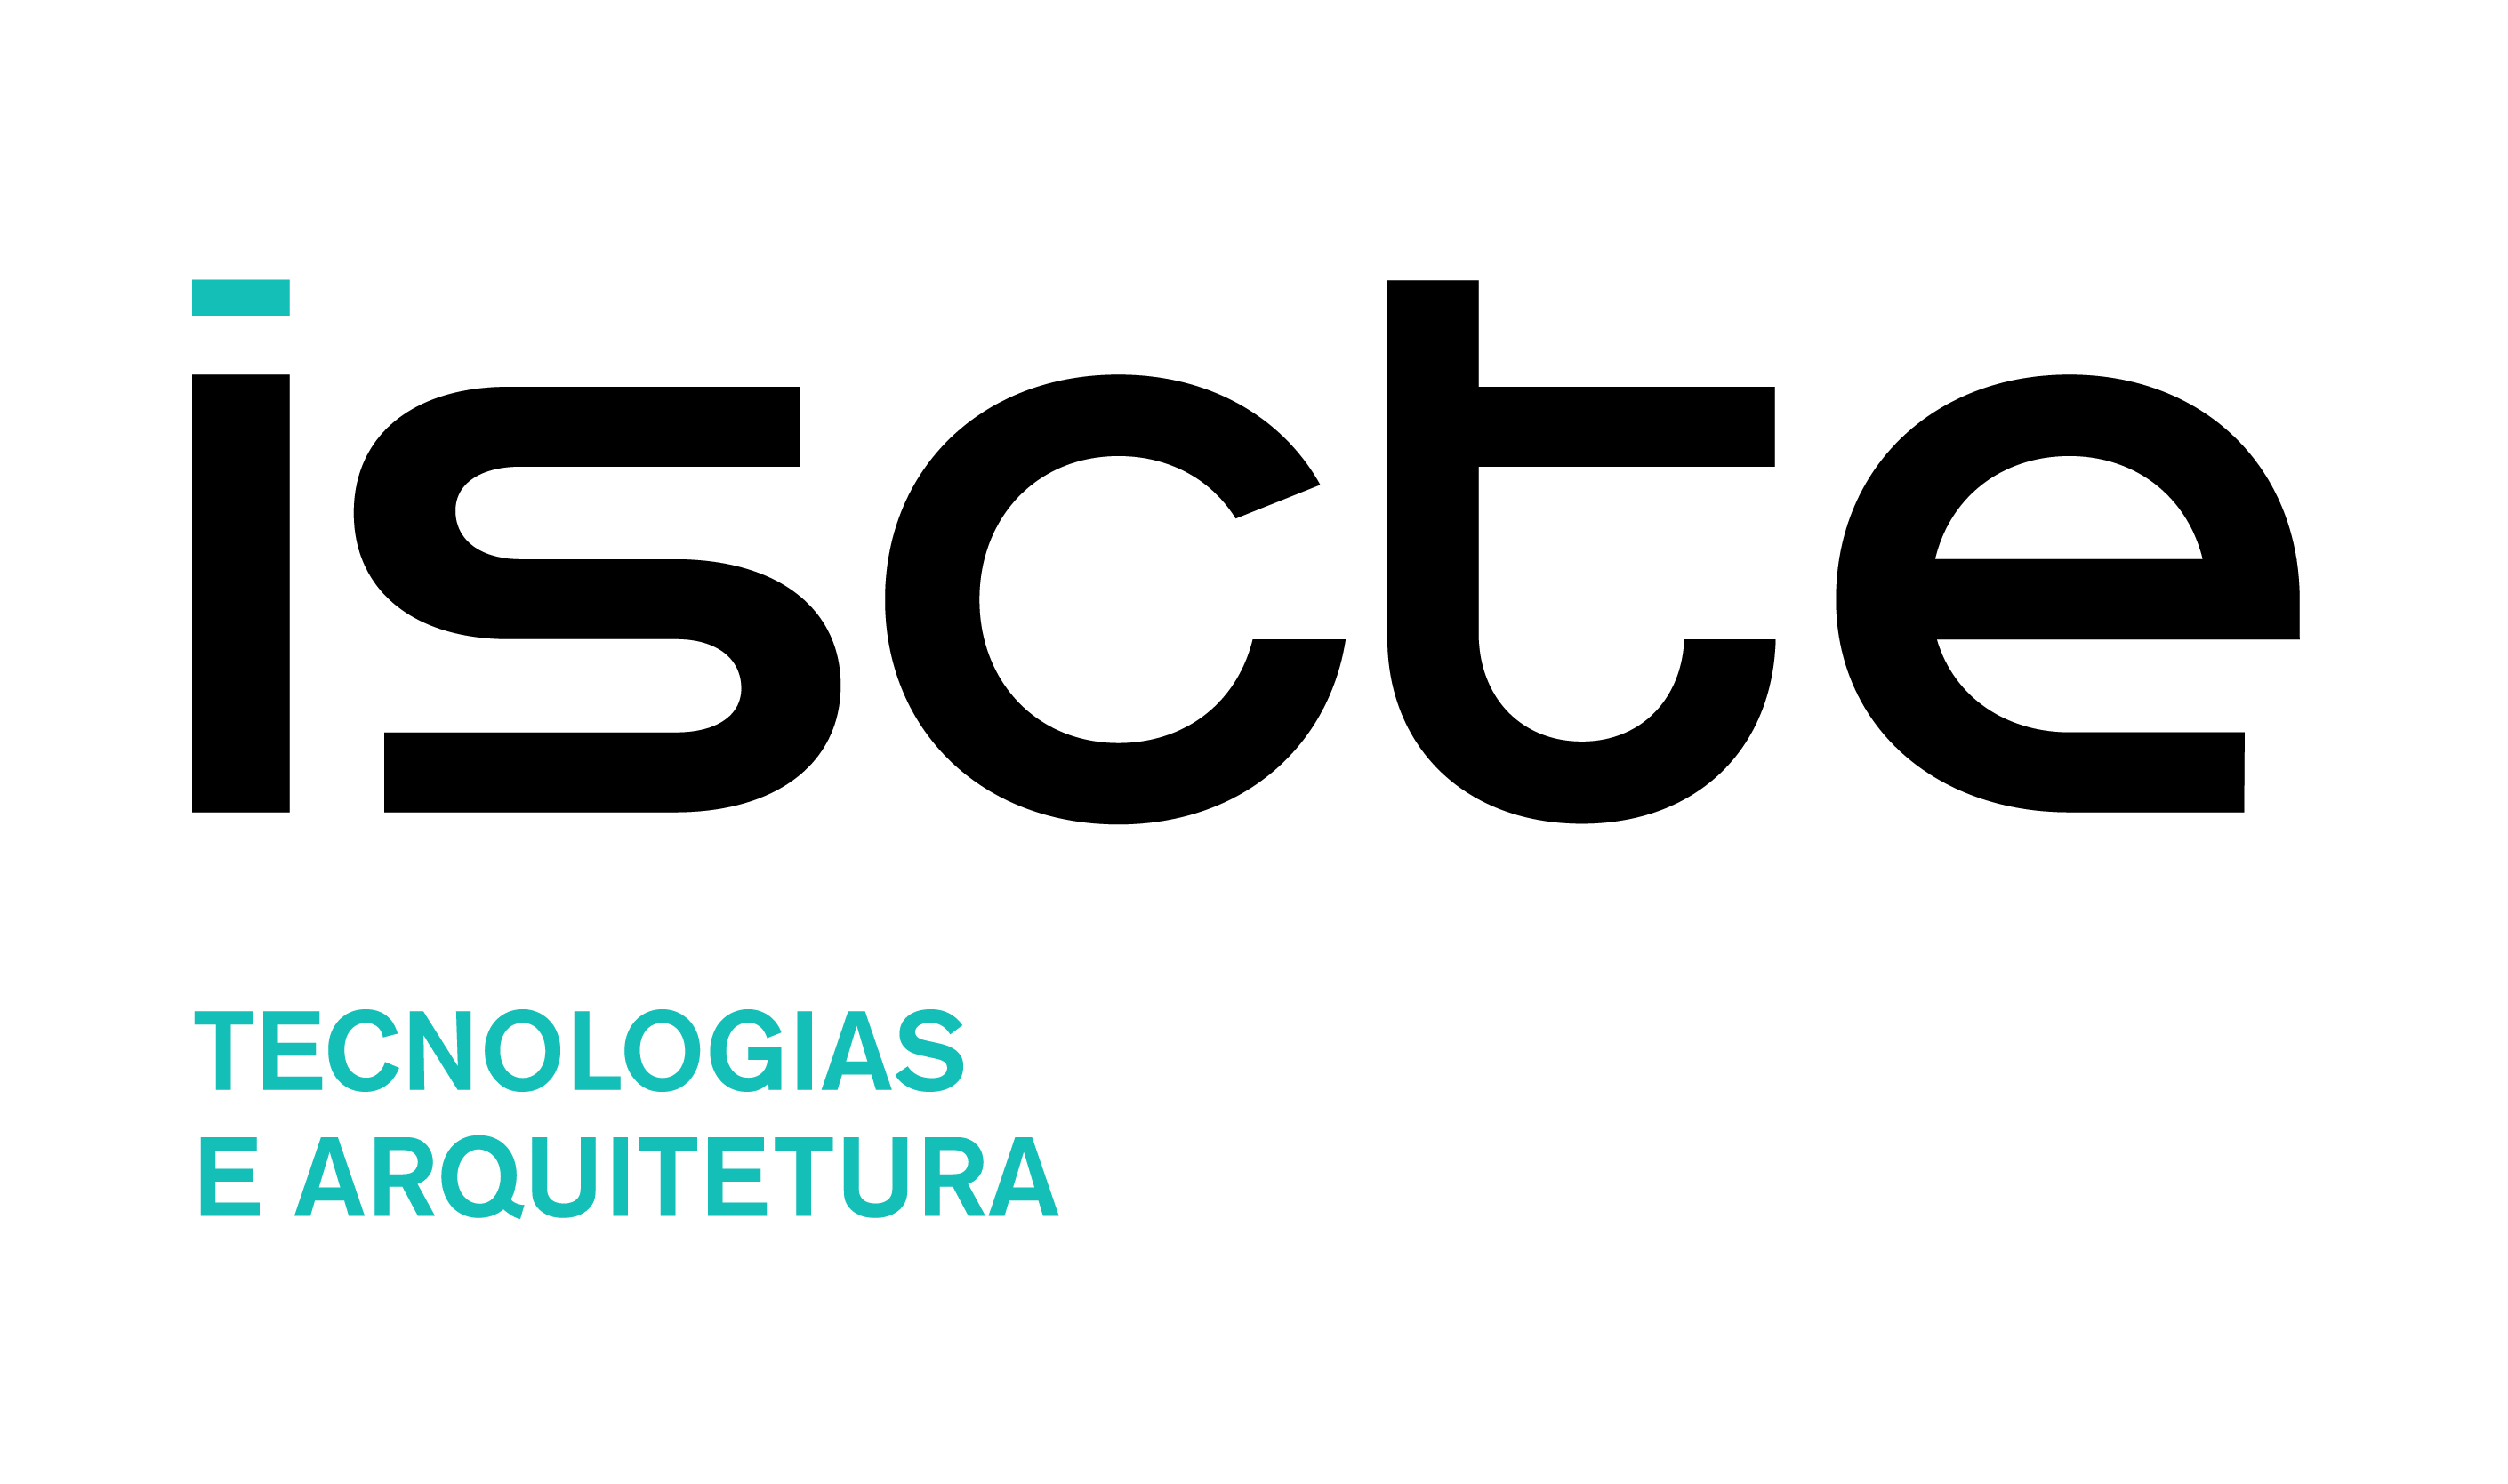
\includegraphics[width=0.5\textwidth]{ista.png}\\[1cm]
		\end{flushleft}
		\noindent
		\textcolor{barraazul}{\rule{\textwidth}{1mm}} % Barra azul
		\\[0.5cm]
		{\Large \textbf{\centering Departamento de Ciências e Tecnologias da Informação}}\\[1cm]
		{\Huge \textbf{\centering Desenvolvimento de modelos preditivos com base em RNN}}\\[1.5cm]
		\noindent
		\textbf{Luís Ricardo Silva Inácio}\\
		\textbf{Número de Aluno: 129074}\\[2cm]
		\textbf{Orientador: Tozé Brito, Phd}\\
		\textbf{Coorientador: (se aplicável)}\\[3cm]
		\textbf{Outubro, 2024}
	\end{titlepage}
	
	% Página de Copyright
	\newpage
	\thispagestyle{empty}
	\noindent
	{\footnotesize % Tamanho menor de texto (menor que \small)
		\textbf{Direitos de cópia ou Copyright} \\ \textcopyright
		Copyright: Luís Ricardo Silva Inácio \\[-0.5cm] % Reduz o espaço após o autor
		\begin{flushleft} % Início do ambiente para alinhar à esquerda e justificar
			\renewcommand{\baselinestretch}{1}\selectfont % Define o espaçamento entre linhas
			\justify % Garante a justificação do texto
			O Iscte - Instituto Universitário de Lisboa tem o direito, perpétuo e sem limites geográficos, de arquivar e publicitar este trabalho através de exemplares impressos reproduzidos em papel ou de forma digital, ou por qualquer outro meio conhecido ou que venha a ser inventado, de o divulgar através de repositórios científicos e de admitir a sua cópia e distribuição com objetivos educacionais ou de investigação, não comerciais, desde que seja dado crédito ao autor e editor.
		\end{flushleft}
	}
	\newpage
	
	% Página de Agradecimentos
	\chapter*{Agradecimentos}
	\addcontentsline{toc}{chapter}{Agradecimentos}
	Gostaria de expressar a minha gratidão a todas as pessoas que me apoiaram durante a realização deste trabalho...
	
	% Resumo
	\newpage
	\chapter*{Resumo}
	\addcontentsline{toc}{chapter}{Resumo}
	Texto do resumo em português. \\[1em]
	\textbf{Palavras-chave:} palavra-chave1, palavra-chave2, palavra-chave3.
	\newpage
	
	% Abstract
	\chapter*{Abstract}
	\addcontentsline{toc}{chapter}{Abstract}
	Texto do resumo em inglês. \\[1em]
	\textbf{Keywords:} keyword1, keyword2, keyword3.
	\newpage
	
	% Índices
	\tableofcontents
	\newpage
	\listoffigures
	\newpage
	\listoftables
	\newpage
	
	% Lista de Abreviaturas e Siglas
	\chapter*{Lista de Abreviaturas e Siglas}
	\addcontentsline{toc}{chapter}{Lista de Abreviaturas e Siglas}
	\begin{longtable}{p{3cm} p{10cm}}
		\textbf{Sigla} & \textbf{Descrição} \\
		\hline
		API & Application Programming Interface \\
		BI & Business Intelligence \\
		KPI & Key Performance Indicator \\
	\end{longtable}
	
	% Começar numeração árabe
	\newpage
	\pagenumbering{arabic}
	
	% Introdução
	\chapter{Introdução}
	A inteligência artificial tem evoluído significativamente nas últimas décadas, com avanços em redes neuronais profundas sendo especialmente notáveis. O livro seminal de \citet{goodfellow2016} destaca como o deep learning transformou o campo, permitindo o desenvolvimento de modelos complexos para problemas de visão computacional, linguagem natural e mais. Além disso, \citet{taylor2015} enfatiza que a simplicidade de certas abordagens pode ser essencial para iniciantes entenderem os fundamentos da aprendizagem automática. 
	
	Os desafios associados à implementação e otimização de redes neuronais foram explorados em várias pesquisas. Por exemplo, \citet{rao2019} argumenta que os principais desafios incluem o ajuste de hiperparâmetros e a escalabilidade dos modelos.
	
	\chapter{Revisão de Literatura}
	A literatura recente tem investigado estratégias para otimizar redes neuronais e melhorar a eficiência dos modelos. \citet{smith2021optimization} analisaram técnicas avançadas de otimização que têm um impacto direto no desempenho de redes neuronais em tarefas críticas. Da mesma forma, \citet{brown2020} exploraram o papel da aprendizagem automática na análise preditiva, destacando a importância do machine learning para setores como saúde e finanças.
	
	Um avanço importante foi a introdução de redes convolucionais para classificação de imagens por \citet{krizhevsky2012}, que revolucionou a área com a sua abordagem baseada no conjunto de dados ImageNet. Estudos subsequentes, como os apresentados em \citet{noauthor2021}, detalham os avanços em redes recorrentes, ampliando sua aplicabilidade em processamento de séries temporais e geração de texto.
	
	Contribuições teóricas também foram fundamentais. O livro \citet{mitpress2018} fornece uma base sólida sobre os princípios de aprendizagem profunda, enquanto \citet{wikipedia2024} oferece uma visão geral acessível das redes neuronais recorrentes.
	
	\chapter{Metodologia}
	A metodologia deste estudo foi baseada em abordagens sugeridas por \citet{smith2021optimization}, que enfatizam a utilização de técnicas otimizadas para treinar redes profundas. Além disso, os parâmetros do modelo foram ajustados com base nos princípios descritos por \citet{rao2019}, garantindo um equilíbrio entre desempenho e complexidade computacional.
	
	O framework experimental foi inspirado nas estratégias utilizadas em \citet{krizhevsky2012}, adaptando redes convolucionais para novos conjuntos de dados. Também foram incorporadas técnicas de análise preditiva baseadas nas metodologias descritas por \citet{brown2020}.
	
	\chapter{Resultados}
	Os resultados obtidos corroboram os achados de \citet{smith2021optimization}, demonstrando melhorias significativas na eficiência do modelo ao adotar técnicas avançadas de otimização. Adicionalmente, os modelos baseados em redes convolucionais apresentaram precisão semelhante às descritas por \citet{krizhevsky2012}, validando sua robustez em tarefas de classificação de imagens.
	
	Curiosamente, as limitações de redes recorrentes, como discutido por \citet{noauthor2021}, foram observadas em tarefas de processamento sequencial, reforçando a necessidade de arquiteturas híbridas para superar esses desafios.
	
	\chapter{Conclusão}
	Com base nas evidências apresentadas, pode-se concluir que a adoção de técnicas modernas de otimização e arquiteturas avançadas de redes neuronais desempenha um papel crucial no avanço da inteligência artificial. Conforme discutido em \citet{goodfellow2016}, o futuro do deep learning depende da contínua integração de métodos teóricos e práticos.
	
	Além disso, as contribuições de \citet{rao2019} e \citet{brown2020} destacam que uma abordagem multidisciplinar é essencial para enfrentar os desafios associados à escalabilidade e aplicação prática dos modelos. Este trabalho, portanto, reforça a importância da pesquisa colaborativa e interdisciplinar no progresso da inteligência artificial.
	
	% Referências
	\printbibliography
	
	% Apêndices
	\appendix
	\chapter{Anexo A}
	Texto fictício para apêndice. 
	\lipsum[10]
	
\end{document}
